
\chapter{Ambiente e Data Mart}
\label{cap:ambiente}

Para esta atividade foi construído um ambiente containerizado
(\textit{Docker Compose}) em cinco camadas, sobre o conjunto de dados abertos
\textit{Sinistros de trânsito agrupados por ocorrência} da \sigla{PRF}{Polícia
Rodoviária Federal} (\textsc{prf-datatran}), publicado no Portal Brasileiro
de Dados Abertos \cite{prfdatatran}: um \sigla{CSV}{Comma-Separated Values}
por ano, 2007 a 2026, uma linha por ocorrência (\texttt{app/dataset/}). A
camada transacional não existe na origem: foi modelada apenas para abstrair
esses arquivos CSV num banco relacional, servindo de fonte para a carga do
DW. O
\autoref{qua:camadas} resume as quatro primeiras camadas; a quinta
(\textit{Machine Learning}, o foco desta atividade) é detalhada no
\autoref{cap:metodologia}.

\begin{figure}[!htb]
  \centering
  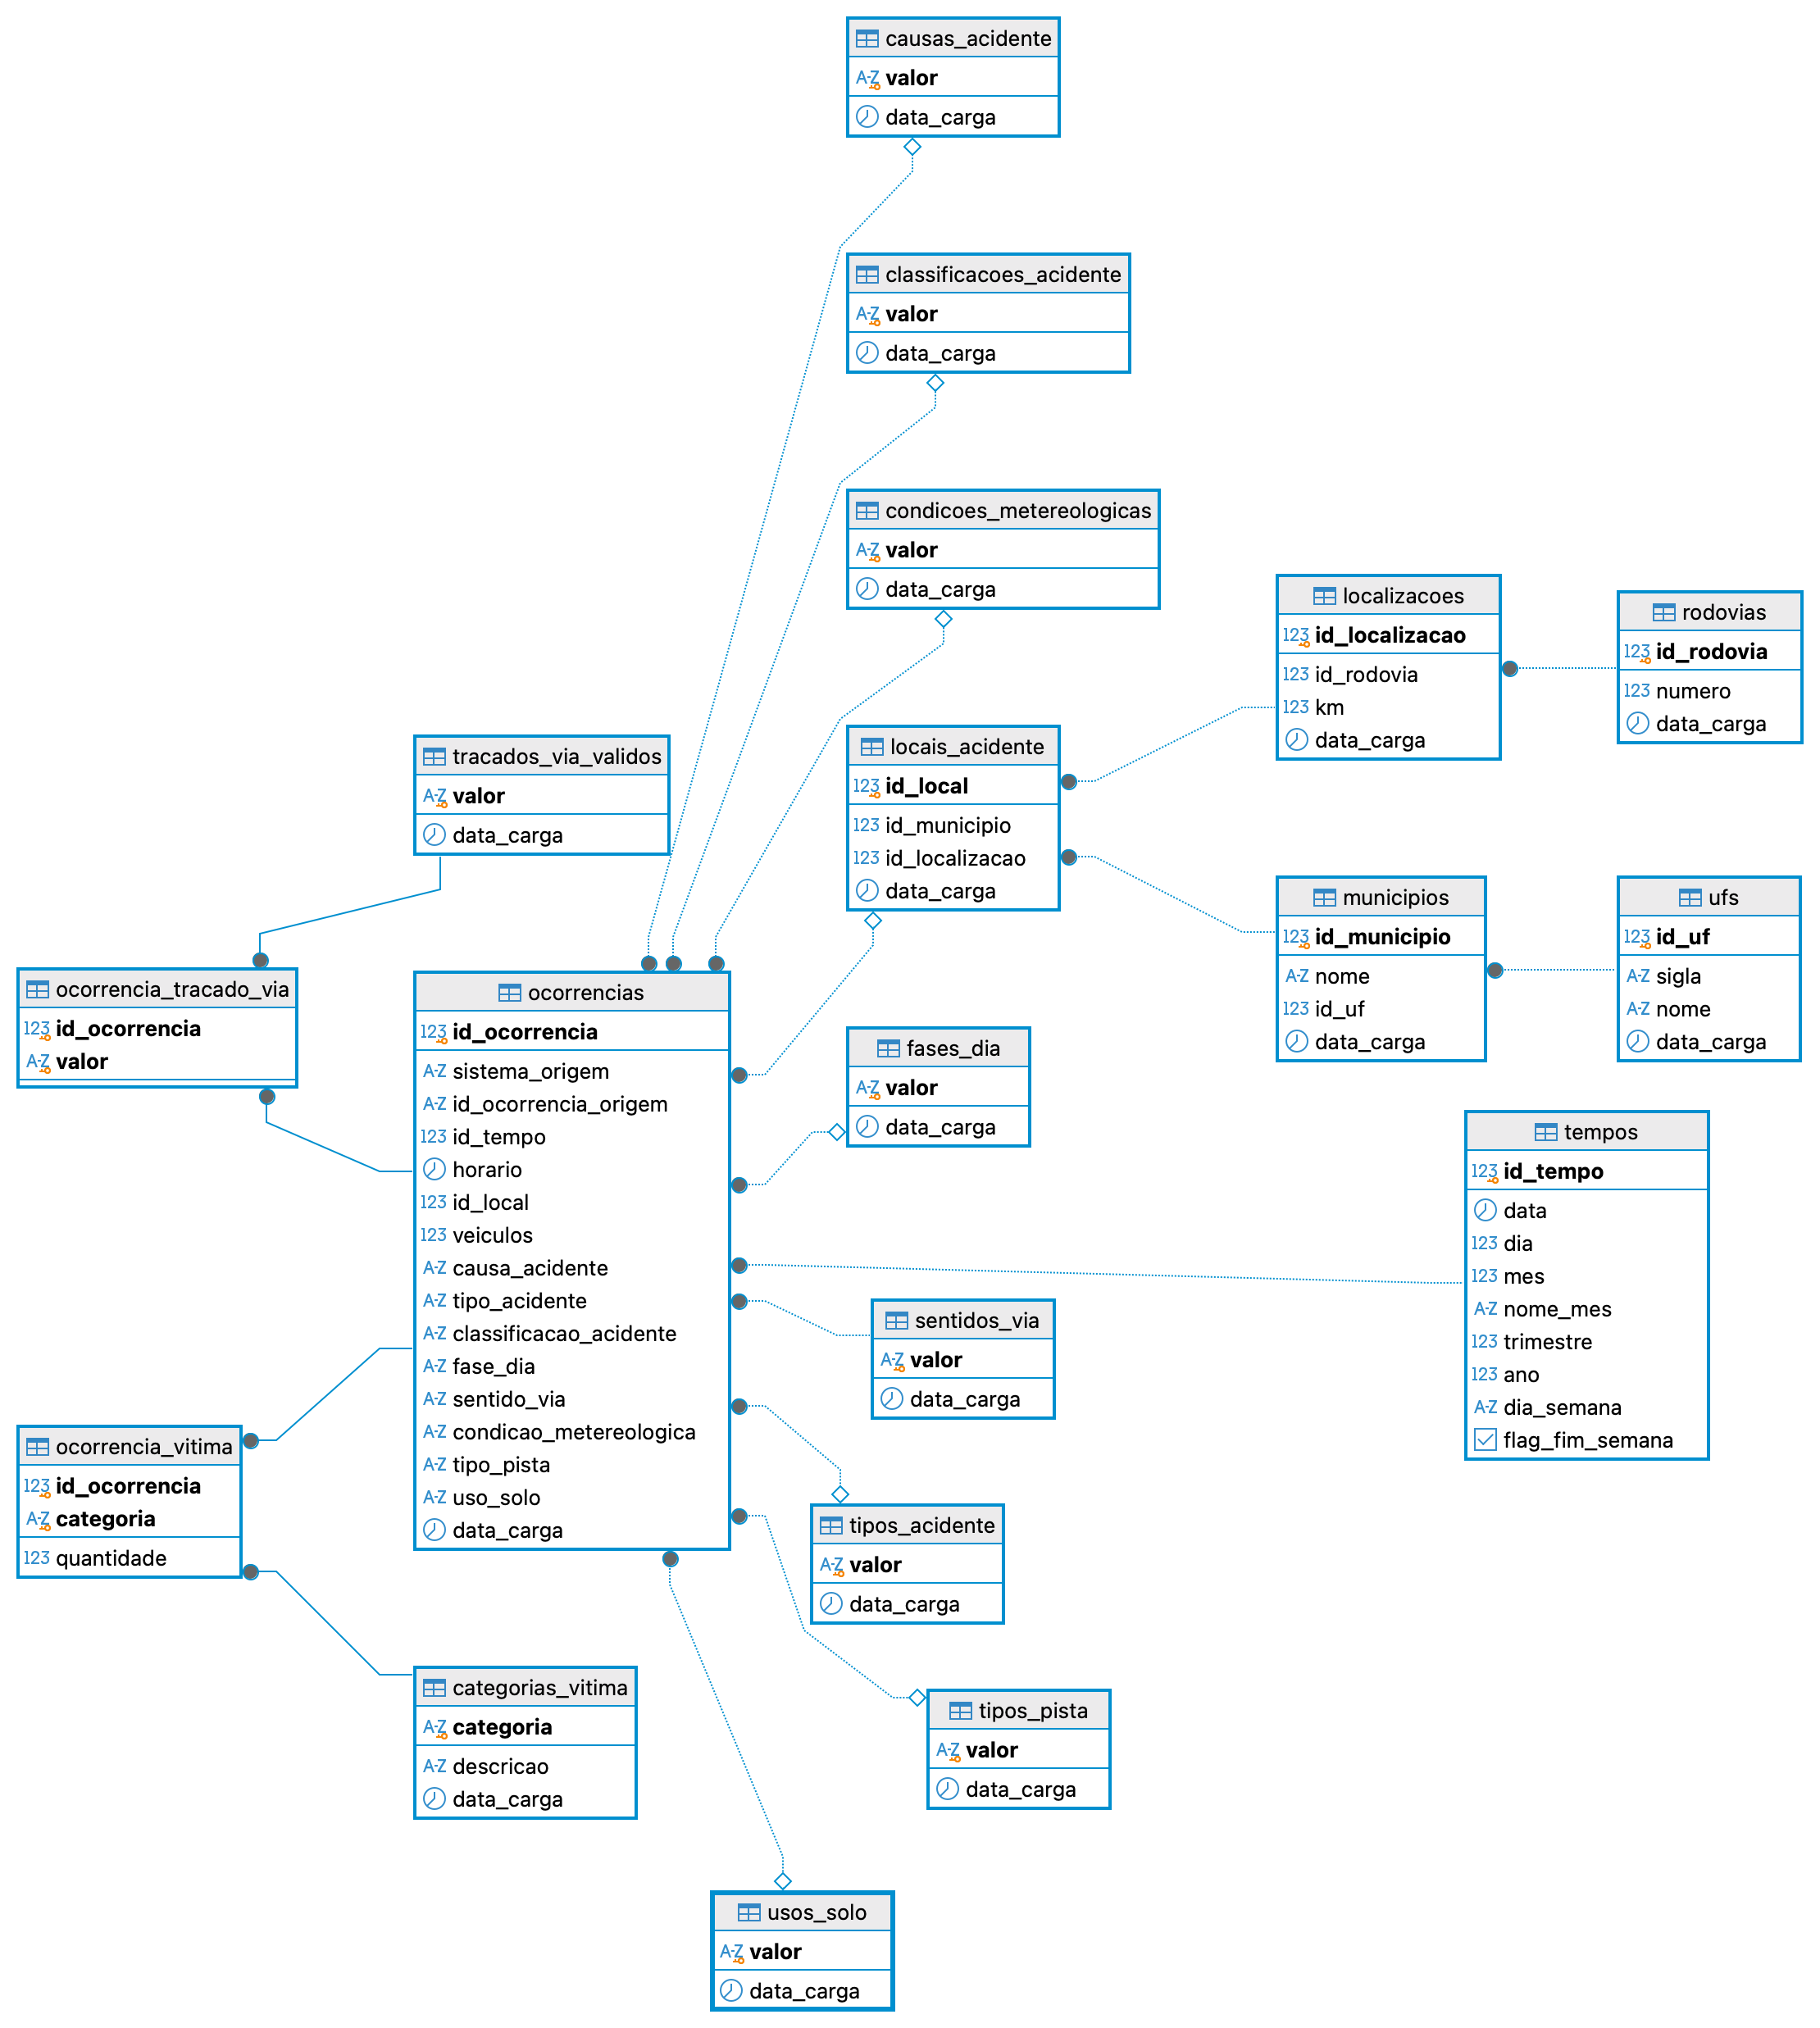
\includegraphics[width=0.75\textwidth]{./fig/dw_corporativo}
  \caption{Diagrama entidade-relacionamento do DW Organizacional (corporativo)}
  \label{fig:dw-corporativo}
  \fontefig{Elaborado pelo autor}
\end{figure}

\begin{quadro}[!ht]
  \centering
  \small
  \caption{Camadas do ambiente construído para esta atividade}
  \label{qua:camadas}
  \begin{tabular}{|p{3.4cm}|p{10.4cm}|}
    \hline
    \textbf{Camada} & \textbf{Descrição} \\
    \hline
    1. Transacional &
    Abstração dos CSV da PRF, normalizada até a 4\textsuperscript{a} Forma
    Normal, banco \texttt{datatran} \\
    \hline
    2. DW corporativo &
    À Inmon \cite{inmon2005} (por assunto, integrado, não-volátil, variante
    no tempo), schema \texttt{corporativo} do banco \texttt{dw} \\
    \hline
    3. Data Mart em estrela &
    À Kimball \cite{kimball2013}, derivado do corporativo, schema
    \texttt{public} do banco \texttt{dw}. Base do \textit{ensemble}
    (\autoref{sec:datamart}) \\
    \hline
    4. BI (Metabase) &
    Painéis via \sigla{API}{Application Programming Interface}, com os
    cards de clusterização e regras de associação (\autoref{sec:bi}) \\
    \hline
  \end{tabular}
  \fontequa{Elaborado pelo autor.}
\end{quadro}

As três primeiras camadas vivem no mesmo servidor PostgreSQL; a carga do
transacional para o DW é feita por duas \sigla{DAG}{Directed Acyclic
Graph}s do Apache Airflow (carga inicial e incremental). O
\autoref{fig:dw-corporativo} mostra o DW Organizacional: por assunto
(Tempo, Geografia, Classificação do Acidente, Vítimas, Ocorrências), cada
catálogo de classificação em tabela própria e \texttt{ocorrencias} como fato
operacional.



\section{Grão e dimensões do Data Mart}
\label{sec:datamart}

Grão de \textbf{1 linha por ocorrência}, sem granularidade por vítima ou
veículo: \texttt{dim\_tempo} (calendário), \texttt{dim\_local} (município,
\sigla{UF}{Unidade da Federação}, rodovia e \textit{km} numa única linha),
\texttt{dim\_classificacao\_acidente} (\textit{dimensão junk} com uma linha
por combinação observada de 8 das 9 classificações da ocorrência) e
\texttt{fato\_acidente\_tracado\_via} (tabela ponte, padrão Kimball, para a
9\textsuperscript{a} classificação, multivalorada desde 2017). O fato
\texttt{fato\_acidentes} traz \texttt{mortos}, \texttt{feridos\_leves},
\texttt{feridos\_graves}, \texttt{ilesos}, \texttt{ignorados} e os totais
pré-calculados \texttt{feridos}/\texttt{pessoas}. O
\autoref{fig:dw-estrela} mostra o diagrama completo do Data Mart em estrela, com as dimensões e o fato.

\begin{figure}[!htb]
  \centering
  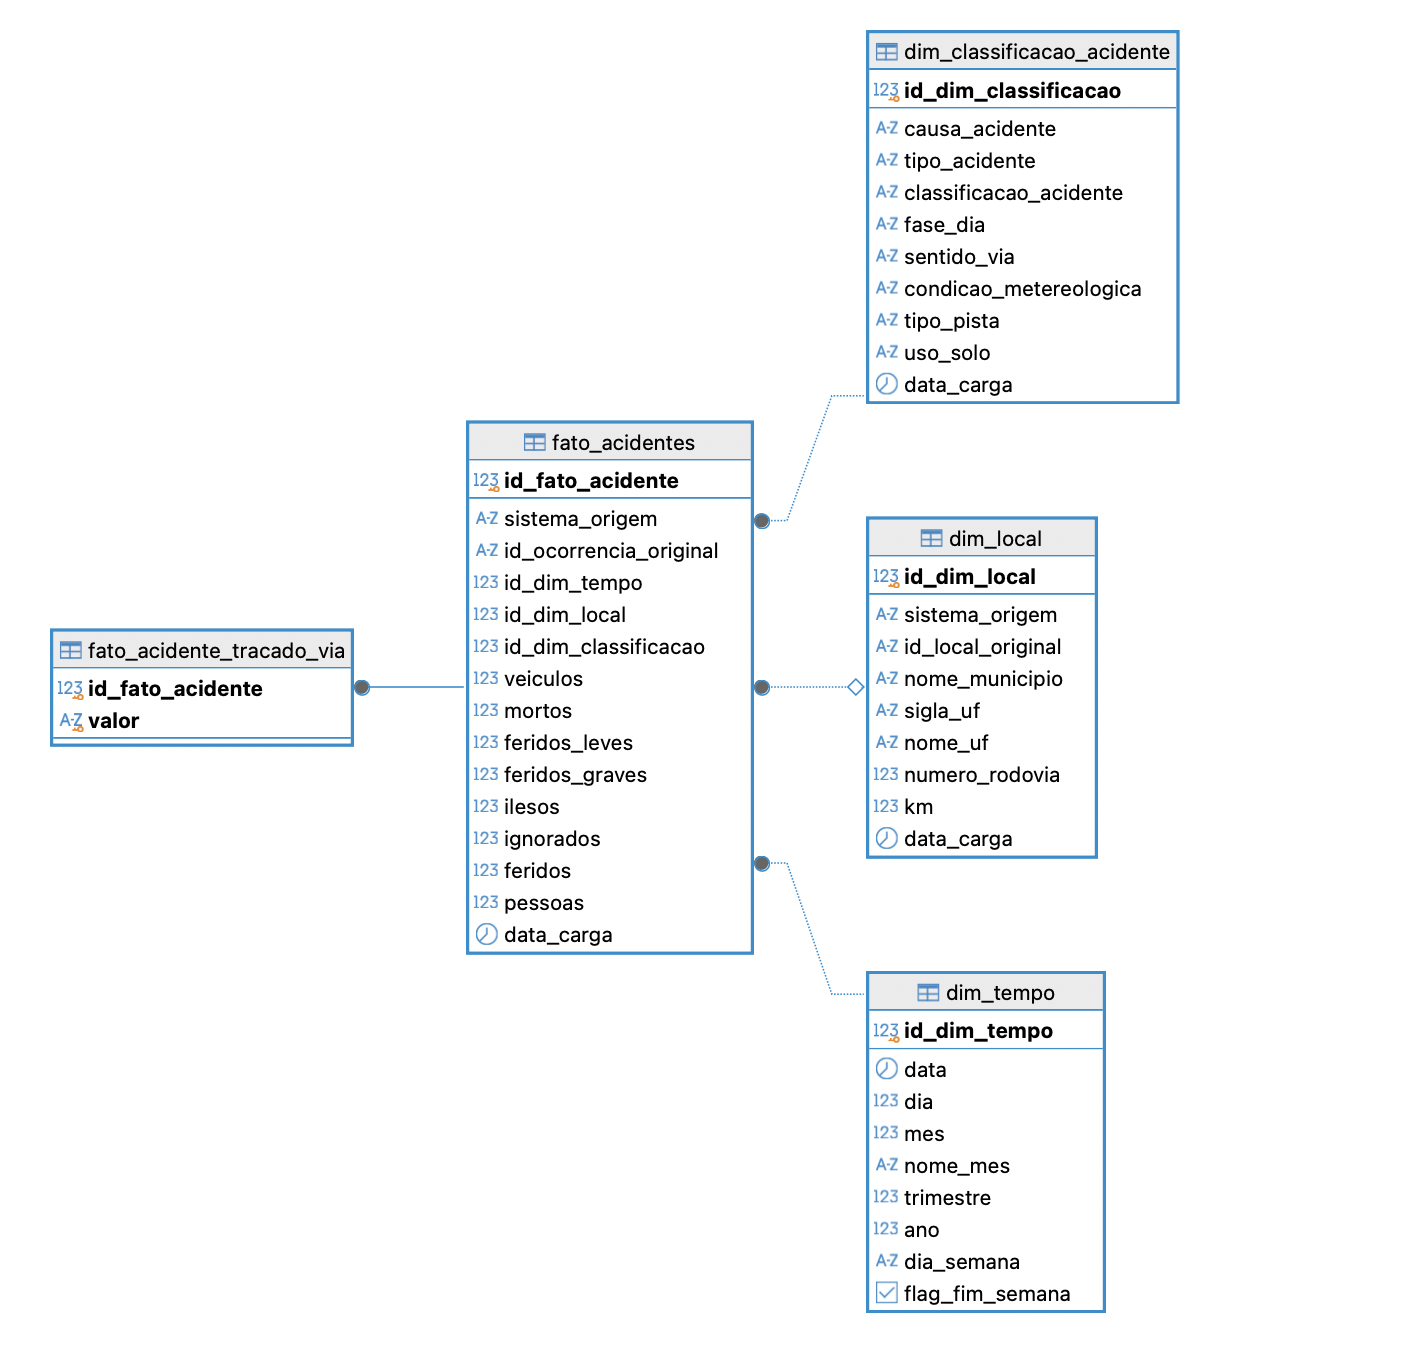
\includegraphics[width=0.75\textwidth]{./fig/dw_martings}
  \caption{Diagrama entidade-relacionamento do Data Mart em estrela}
  \label{fig:dw-estrela}
  \fontefig{Elaborado pelo autor}
\end{figure}

\section{Catálogo de metadados}
\label{sec:metadados}

Um schema \texttt{metadados} (\autoref{fig:dw-metadados}) documenta a
origem e a regra de transformação de cada campo do DW: tabelas/campos do
transacional, do corporativo/Data Mart, algoritmos de
\sigla{ETL}{Extract, Transform, Load} e a linhagem entre eles. Fica
navegável como dicionário de dados num painel próprio do Metabase.

\begin{figure}[!htb]
  \centering
  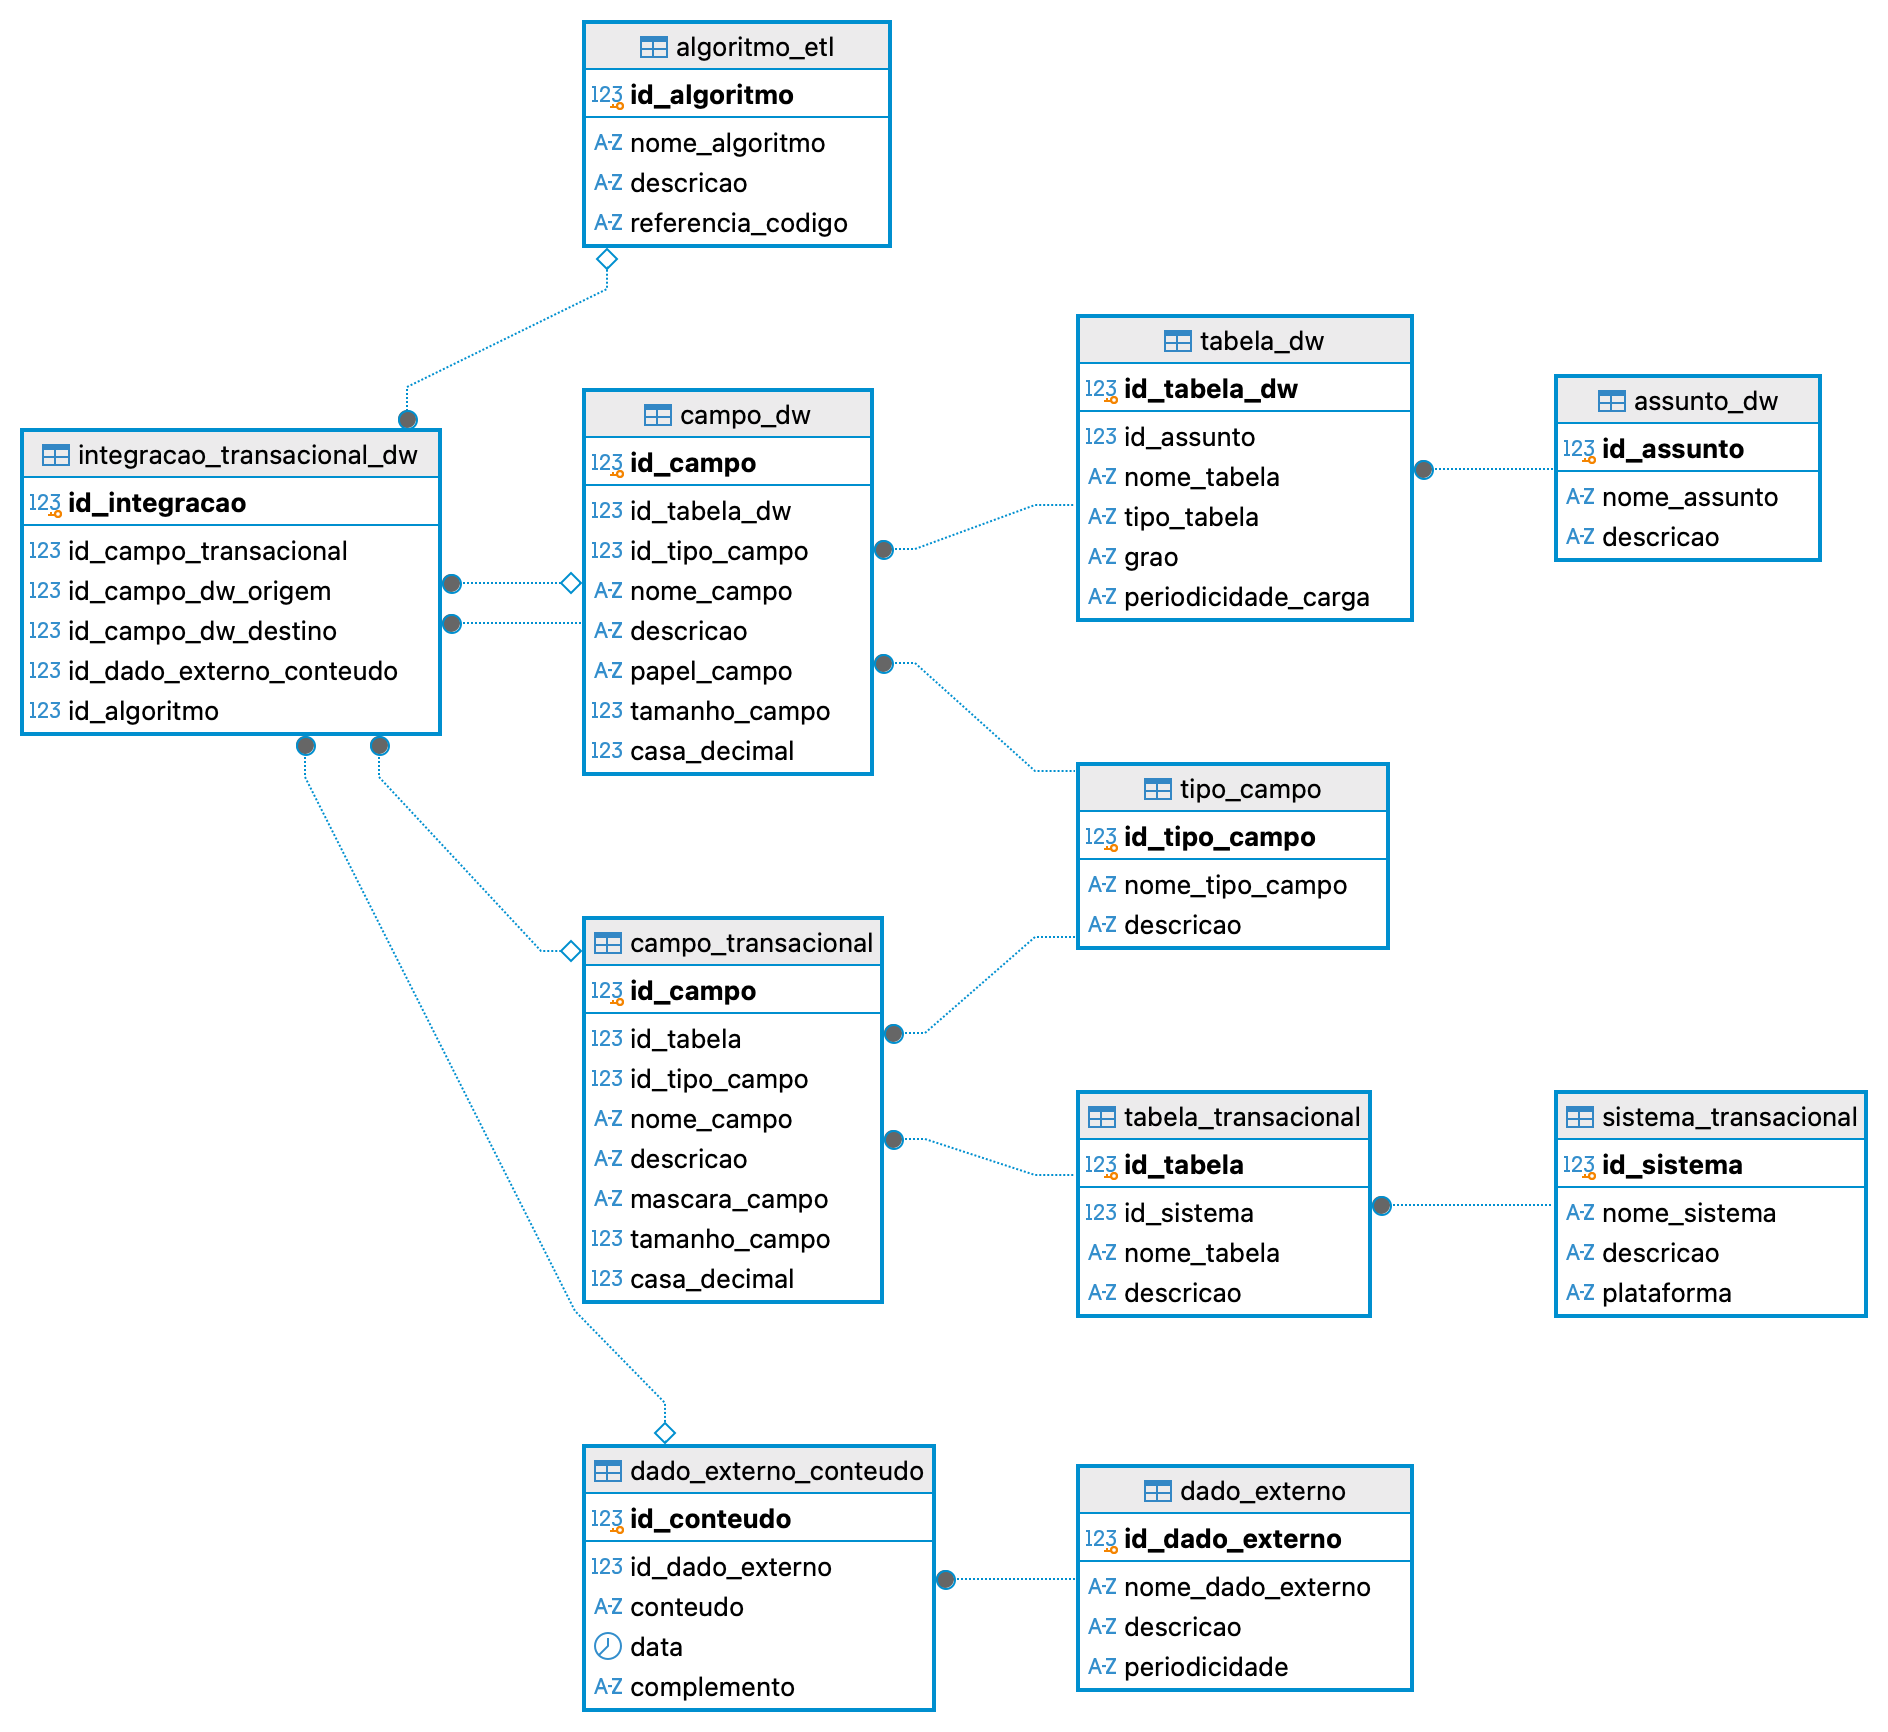
\includegraphics[width=0.75\textwidth]{./fig/dw_metadados}
  \caption{Diagrama entidade-relacionamento do catálogo de metadados}
  \label{fig:dw-metadados}
  \fontefig{Elaborado pelo autor}
\end{figure}
